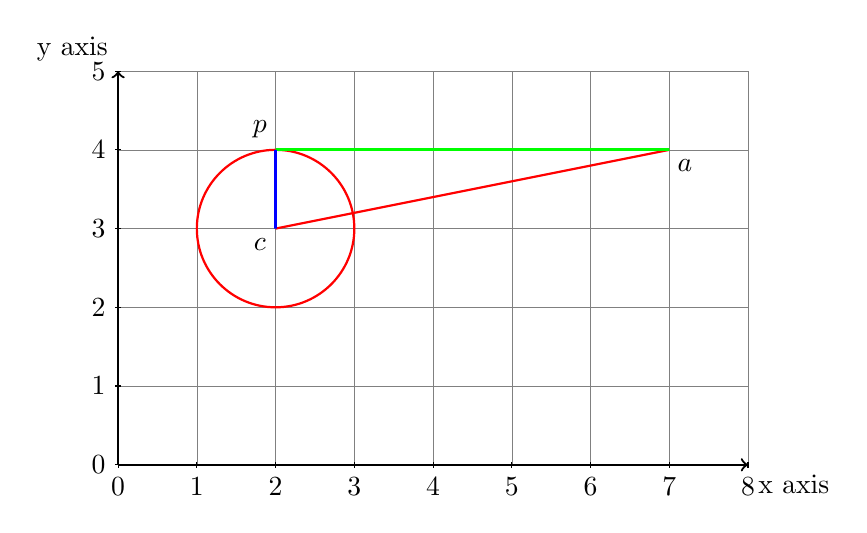
\begin{tikzpicture}
[
	scale=1,
	point/.style = {draw, circle, fill=green, inner sep=0.5pt},
]
\draw[step=1cm,gray,very thin] (0,0) grid (8,5);		

\draw[red,thick] (2,3) circle (1 cm);
\draw (1.8,3) node[anchor=north]{$c$};		
\draw (1.8,4.5) node[anchor=north]{$p$};


\draw (7.2,4) node[anchor=north]{$a$};
\draw[red][thick] (2,3) -- (7,4) 	-- cycle;
\draw[green][very thick] (2,4) -- (7,4) 	-- cycle;
\draw[blue][very thick] (2,3) -- (2,4) 	-- cycle;	
	
\draw[thick,->] (0,0) -- (8,0) node[anchor=north west] {x axis};
\draw[thick,->] (0,0) -- (0,5) node[anchor=south east] {y axis};
\foreach \x in {0,1,2,3,4,5,6,7,8}
\draw (\x cm,1pt) -- (\x cm,-1pt) node[anchor=north] {$\x$};
\foreach \y in {0,1,2,3,4,5}
\draw (1pt,\y cm) -- (-1pt,\y cm) node[anchor=east] {$\y$};
\end{tikzpicture}
